\documentclass[tikz]{standalone}
\usepackage[T1]{fontenc}
\usepackage[utf8]{inputenc}
\usepackage{pgfplots}
\usepackage{grffile}
\pgfplotsset{compat=newest}
\usetikzlibrary{plotmarks}
\usetikzlibrary{arrows.meta}
\usepgfplotslibrary{patchplots}
\usepackage{amsmath}

\begin{document}
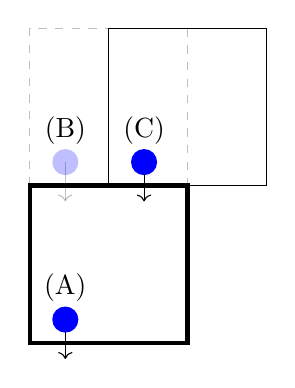
\begin{tikzpicture}


\path[draw,ultra thick] (0,0) rectangle (2,2);
\path[draw,dashed,opacity=0.25] (0,2) rectangle (2,4);
\path[draw] (1,2) rectangle (3,4);
\draw[->](0.45,0.3)--(0.45,-0.2);
\draw[->,opacity=0.25](0.45,2.3)--(0.45,1.8);
\draw[->](1.45,2.3)--(1.45,1.8);
\node[circle, fill=blue] at (0.45,0.3) {};
\node[circle, fill=blue,opacity=0.25] at (0.45,2.3) {};
\node[circle, fill=blue] at (1.45,2.3) {};

\node at (0.45,0.7) {(A)};
\node at (0.45,2.7) {(B)};
\node at (1.45,2.7) {(C)};
\end{tikzpicture}%
\end{document}